\documentclass[10pt,twocolumn]{article}

\usepackage[margin=0.72in,columnsep=0.24in]{geometry}
\usepackage[T1]{fontenc}
\usepackage[utf8]{inputenc}
\usepackage{lmodern}
\usepackage{microtype}
\usepackage{balance}
\usepackage{amsmath,amssymb}
\usepackage{booktabs}
\usepackage{tabularx}
\usepackage{graphicx}
\usepackage{tikz}
\usepackage{enumitem}
\usepackage{xcolor}
\usepackage{xurl}
\usepackage{seqsplit}
\usepackage{hyperref}
\usepackage[capitalise,noabbrev]{cleveref}
\usetikzlibrary{arrows.meta,positioning,fit,backgrounds}

\definecolor{FBBlue}{HTML}{1769AA}
\definecolor{FBGold}{HTML}{E6A11A}
\definecolor{FBTeal}{HTML}{168C7A}
\definecolor{FBRed}{HTML}{C75450}
\definecolor{FBCharcoal}{HTML}{262B33}
\definecolor{FBPaper}{HTML}{F7F8FA}
\hypersetup{
  colorlinks=true,
  linkcolor=FBBlue,
  citecolor=FBBlue,
  urlcolor=FBBlue,
  pdftitle={FlavourBench: Epicure as an Executable Oracle for Ranking Culinary Agents},
  pdfauthor={Josef Chen},
  pdfsubject={An automated benchmark and paired tool-uplift study for frontier culinary agents},
  pdfkeywords={language models, benchmarks, tool use, culinary reasoning, reinforcement learning}
}
\setlist{leftmargin=*,nosep}
\setlength{\parindent}{1em}
\setlength{\parskip}{0pt}

\newcommand{\system}{\textsc{FlavourBench}}
\newcommand{\epicure}{\textsc{Epicure}}
\newcommand{\sha}[1]{\texttt{\seqsplit{#1}}}
\newcommand{\FBReleaseSHA}{\texttt{603e4aa4db86\ldots}}
\newcommand{\FBModels}{20}
\newcommand{\FBTasks}{32}
\newcommand{\FBPairs}{640}
\newcommand{\FBArms}{1280}
\newcommand{\FBObservedArms}{1195}
\newcommand{\FBMissingArms}{85}
\newcommand{\FBTopModel}{GPT-5.6 Sol Pro}
\newcommand{\FBTopScore}{62.5}
\newcommand{\FBTopCorrect}{20}
\newcommand{\FBTopOnCorrect}{32}
\newcommand{\FBTopUplift}{+37.5}
\newcommand{\FBBottomModel}{Nemotron 3 Ultra}
\newcommand{\FBBottomScore}{0.0}
\newcommand{\FBBottomCorrect}{0}
\newcommand{\FBAggregateOff}{43.9}
\newcommand{\FBAggregateOn}{93.9}
\newcommand{\FBAggregateUplift}{+50.0}
\newcommand{\FBToolCalls}{606}
\newcommand{\FBReferenceMatches}{606}
\newcommand{\FBObservedCost}{5.19}
\newcommand{\FBPositiveUpliftModels}{19}
\newcommand{\FBNegativeUpliftModels}{0}
\newcommand{\FBZeroUpliftModels}{1}
\newcommand{\FBBestUpliftModel}{Mistral Large 2512}
\newcommand{\FBBestUplift}{+93.8}
\newcommand{\FBWorstUpliftModel}{Nemotron 3 Ultra}
\newcommand{\FBWorstUplift}{+0.0}
\newcommand{\FBWorstBaseReliabilityModels}{Mistral Large 2512 and Nemotron 3 Ultra}
\newcommand{\FBWorstBaseReliability}{0.0}
\newcommand{\FBCoherePlusRank}{16}
\newcommand{\FBCohereReasoningRank}{12}
\newcommand{\FBCoherePlusScore}{40.6}
\newcommand{\FBCoherePlusUplift}{+59.4}
\newcommand{\FBCohereReasoningScore}{46.9}
\newcommand{\FBCohereReasoningUplift}{+50.0}
\newcommand{\FBKimiRank}{5}
\newcommand{\FBQwenRank}{11}
\newcommand{\FBGLMRank}{15}


\title{\vspace{-1.4em}\system{}: Epicure as an Executable Oracle\\
for Ranking Culinary Agents}
\author{Josef Chen\\\small Independent Researcher}
\date{August 2026}

\begin{document}
\raggedbottom
\twocolumn[
  \begin{@twocolumnfalse}
  \maketitle
  \vspace{-1.1em}
  \begin{abstract}
  Culinary reasoning is usually evaluated with broad preference judgments or static question
  banks. Both make it difficult to separate remembered food knowledge from the ability to query a
  domain system and use its result. We introduce \system{}, an automated benchmark built from the
  versioned \epicure{} ingredient runtime. \epicure{} deterministically compiles four families of
  multiple-choice tasks---nearest-neighbour substitution, exact pairing affinity, flavour-axis
  comparison, and cuisine projection---together with their answer keys. No language model writes
  or judges a task.

  We evaluate \FBModels{} frontier models on the same \FBTasks{} tasks in two matched conditions:
  model alone and model with read-only \epicure{} access. The release contains \FBPairs{} paired
  trials and \FBArms{} scored arms. \FBTopModel{} ranks first with an Epicure Benchmark Score of
  \FBTopScore{}, while \FBBottomModel{} scores \FBBottomScore{}. Across the panel, tool access
  changes exact-choice accuracy from \FBAggregateOff\% to \FBAggregateOn\%
  (\FBAggregateUplift{} percentage points). The paired design therefore provides both a conventional
  model ranking and a direct estimate of domain-tool uplift.

  The benchmark is fully replayable from a single content-addressed release containing the task
  compiler outputs, answer keys, routes, final responses, and projected tool traces. Beyond
  evaluation, the same exact reward can support rejection sampling, preference construction, and
  reinforcement learning. \system{} turns a culinary knowledge system into an executable oracle:
  it measures what a model knows, what it can retrieve, and whether tool access actually improves
  the answer.
  \end{abstract}
  \vspace{0.5em}
  \end{@twocolumnfalse}
]

\section{Introduction}

Benchmarks are easiest to trust when their ground truth is external to the models being tested.
Code can be executed, database states can be inspected, and games can be scored. Culinary
reasoning rarely has that luxury. Ingredient substitutions, pairings, technique choices, and
cuisine associations are commonly assessed by another language model or by a small set of human
preferences. The evaluator then becomes part of the construct.

\system{} takes a different route. It starts from \epicure{}, a read-only culinary runtime with
1,790 ingredients represented in a 300-dimensional space \cite{radzikowski2026structure,
radzikowski2026geometry}. The benchmark calls four deterministic
operations, converts their results into four-choice questions, and records the exact answer before
any evaluated model is contacted. The resulting task is compact enough to rerun whenever the
frontier changes, yet structured enough to expose different kinds of culinary reasoning.

The experimental design asks two questions at once. First, how accurately can a model recover
\epicure{}'s answers without access to the runtime? This is the public model ranking. Second, what
changes when the same model receives the exact read-only operation needed to solve the task? This
is the paired tool-uplift experiment. Every model sees every task in both conditions, so differences
are not confounded by task allocation.

Our release evaluates \FBModels{} current endpoints, including GPT-5.6 Sol, Terra, and Luna;
Claude Fable, Opus, and Sonnet 5; Gemini 3.1 Pro and 3.6 Flash; Grok 4.5; Kimi K3; Qwen 3.8 Max;
GLM 5.2; two DeepSeek V4 variants; MiniMax M3; Nemotron 3 Ultra; Mistral Large 2512; Tencent HY 3;
and Cohere Command A Plus and Command A Reasoning. Kimi and both Cohere models use direct provider
routes. Every other endpoint uses an exact, no-fallback OpenRouter route selected before the run.

The paper makes four contributions:

\begin{enumerate}[label=\arabic*.]
  \item an automated culinary benchmark whose questions and answer keys are generated by a
  versioned executable oracle rather than a model judge;
  \item a common-task frontier evaluation with \FBPairs{} matched pairs, exact missing-response
  penalties, and a public 20-row leaderboard;
  \item a matched tool-access comparison that reports both aggregate uplift and model--family
  interactions; and
  \item a training interface that converts the same deterministic reward into rejection sampling,
  pairwise preference data, or reinforcement learning signals.
\end{enumerate}

The headline outcome is concrete: \epicure{} is used twice, first to create the benchmark and then
as the intervention being measured. That makes the same culinary system both an evaluation oracle
and a measurable tool intervention.

\begin{figure*}[t]
  \centering
  \resizebox{\linewidth}{!}{%
  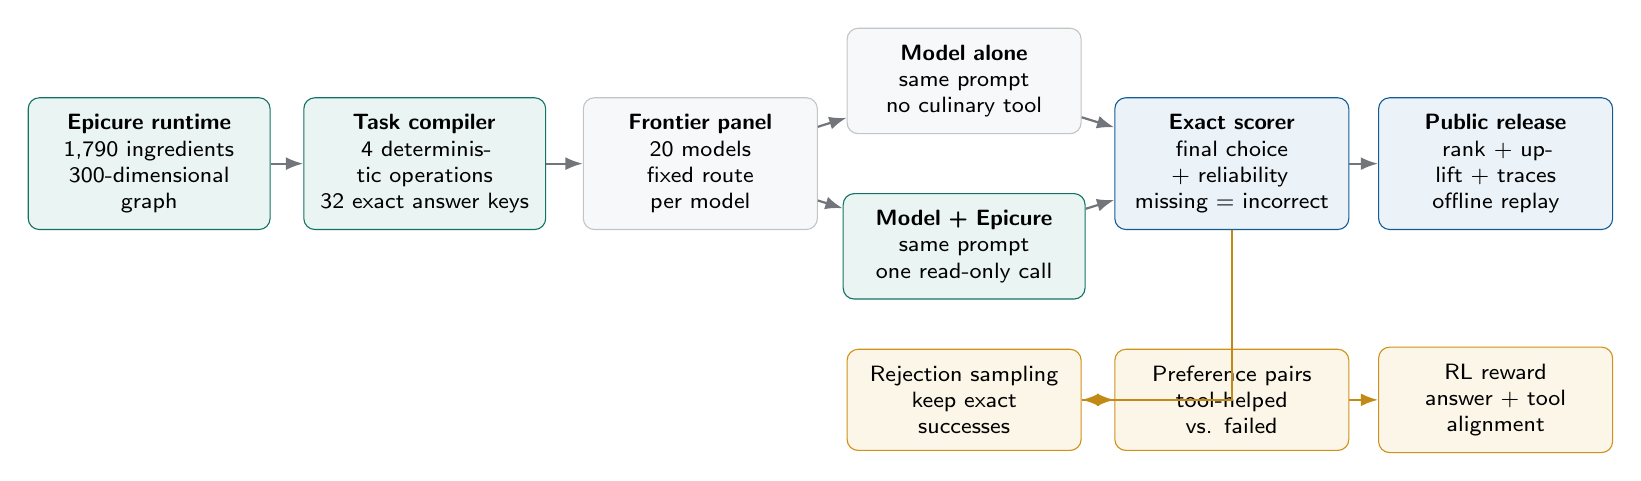
\begin{tikzpicture}[
    x=1cm,y=1cm,font=\sffamily\footnotesize,
    box/.style={draw=FBCharcoal!28,rounded corners=4pt,fill=FBPaper,
      minimum height=1.22cm,text width=2.55cm,align=center,inner sep=6pt},
    oracle/.style={draw=FBTeal!82!black,rounded corners=4pt,fill=FBTeal!9,
      minimum height=1.22cm,text width=2.65cm,align=center,inner sep=6pt},
    score/.style={draw=FBBlue!88!black,rounded corners=4pt,fill=FBBlue!8,
      minimum height=1.22cm,text width=2.55cm,align=center,inner sep=6pt},
    train/.style={draw=FBGold!90!black,rounded corners=4pt,fill=FBGold!10,
      minimum height=1.08cm,text width=2.55cm,align=center,inner sep=6pt},
    arrow/.style={-{Latex[length=2.2mm]},thick,draw=FBCharcoal!65}
  ]
    \node[oracle] (graph) at (0,0) {\textbf{Epicure runtime}\\1,790 ingredients\\300-dimensional graph};
    \node[oracle] (compiler) at (3.5,0) {\textbf{Task compiler}\\4 deterministic operations\\32 exact answer keys};
    \node[box] (panel) at (7.0,0) {\textbf{Frontier panel}\\20 models\\fixed route per model};
    \node[box] (off) at (10.35,1.05) {\textbf{Model alone}\\same prompt\\no culinary tool};
    \node[oracle] (on) at (10.35,-1.05) {\textbf{Model + Epicure}\\same prompt\\one read-only call};
    \node[score] (scorer) at (13.75,0) {\textbf{Exact scorer}\\final choice + reliability\\missing = incorrect};
    \node[score] (release) at (17.1,0) {\textbf{Public release}\\rank + uplift + traces\\offline replay};
    \node[train] (rs) at (10.35,-3.0) {Rejection sampling\\keep exact successes};
    \node[train] (pref) at (13.75,-3.0) {Preference pairs\\tool-helped vs. failed};
    \node[train] (rl) at (17.1,-3.0) {RL reward\\answer + tool alignment};

    \draw[arrow] (graph) -- (compiler);
    \draw[arrow] (compiler) -- (panel);
    \draw[arrow] (panel) -- (off);
    \draw[arrow] (panel) -- (on);
    \draw[arrow] (off) -- (scorer);
    \draw[arrow] (on) -- (scorer);
    \draw[arrow] (scorer) -- (release);
    \draw[arrow,draw=FBGold!85!black] (scorer) |- (rs);
    \draw[arrow,draw=FBGold!85!black] (rs) -- (pref);
    \draw[arrow,draw=FBGold!85!black] (pref) -- (rl);
  \end{tikzpicture}}
  \caption{\system{} turns \epicure{} into an executable oracle. The upper path is the released
  benchmark: deterministic task construction, matched model calls, exact scoring, and offline
  replay. The lower path reuses the same score as training data without introducing an LLM judge.}
  \label{fig:architecture}
\end{figure*}

\section{Epicure-native ground truth}
\label{sec:oracle}

\subsection{A versioned executable oracle}

The evaluated target is not a chef's universal preference. It is the output of a specific,
versioned culinary computation. The release binds an \epicure{} application hash, evidence-bundle
hash, release identifier, ingredient count, and embedding dimensionality. Rebuilding the task set
against a different runtime necessarily produces a different task-set hash.

This definition is narrow by design. It makes every answer independently recomputable and allows
models to be compared without asking another model which response sounds better. It also gives the
score a direct interpretation: accuracy is agreement with the executable culinary model under the
published task construction.

\subsection{Four balanced task families}

The compiler creates eight tasks in each of four families. Seeds and ingredient pairs are fixed
before evaluation. For every task, \epicure{} is called once to obtain the reference result. The
correct answer is extracted programmatically, three distractors are constructed without model
generation, and the four options are shuffled with a task-ID-derived seed.

\begin{table*}[t]
  \centering
  \small
  \begin{tabularx}{\linewidth}{@{}l l X X r@{}}
    \toprule
    Family & Epicure operation & Exact target & Example query & Tasks \\
    \midrule
    Substitution & \texttt{neighbors} & first ranked neighbour & top neighbour for tomato & 8 \\
    Composition & \texttt{pairing\_score} & four-decimal affinity & tomato + basil & 8 \\
    Cookability & \texttt{compare\_on\_axis} & larger flavour projection & coffee vs. chocolate on bitter & 8 \\
    Evidence & \texttt{cultural\_profile} & highest cuisine cosine & cuisine direction for kimchi & 8 \\
    \bottomrule
  \end{tabularx}
  \caption{The task set is balanced by construction. Each family maps one deterministic \epicure{}
  operation to a four-choice answer. Chance accuracy is 25\%.}
  \label{tab:tasks}
\end{table*}

The task families deliberately mix retrieval and computation. Neighbour and cuisine questions test
whether a model knows relationships encoded by the graph. Pairing questions require an exact
numeric result that is difficult to guess. Axis questions test a comparative claim rather than a
memorised scalar. Together they prevent the leaderboard from reducing to one operation or one
kind of culinary trivia.

\subsection{Prompt and answer contract}

Each prompt names the relevant operation and gives four choices. Models may explain briefly, but
the last answer line must be \texttt{FINAL\_CHOICE: X}. The parser accepts exactly one of A--D on
that marker line. A missing marker, abnormal provider finish, timeout, or absent response scores
zero. The rule is intentionally simple enough to implement in a standalone verifier.

The complete task set contains no hidden human label and no model-authored item. The benchmark is
therefore suitable for automatic reruns, CI-style regression tests, and training loops where
thousands of candidate responses must be scored consistently.

\section{Evaluation design}
\label{sec:design}

\subsection{Matched tool-off and tool-on arms}

For model $m$, task $t$, and condition $c\in\{0,1\}$, let $Y_{mtc}$ equal one when the response
finishes normally and its final choice matches the \epicure{} answer key. Condition $c=0$ removes
the tool catalog; condition $c=1$ exposes a minimal read-only \epicure{} call contract. The prompt,
route, temperature, top-$p$, seed request, output limit, and answer parser are otherwise identical.

Each tool-enabled arm may make one successful culinary call. The runner records the tool name,
arguments, latency, error flag, and a hash of the returned payload. Tool output is bounded before it
is appended to model context. Automatic provider fallback is disabled: a route failure remains a
failure for that route.

The model-alone benchmark score is
\begin{equation}
 S_m = 100\,\frac{1}{4}\sum_{f=1}^{4}\frac{1}{8}
       \sum_{t\in f}Y_{mt0}.
 \label{eq:score}
\end{equation}
Because every family contains eight tasks, this equals ordinary accuracy over 32 tasks while making
the intended family weighting explicit. The public rank sorts by $S_m$, then by tool-enabled
accuracy, tool-enabled parse reliability, and model ID.

Tool uplift is the matched difference
\begin{equation}
 U_m = 100\,\frac{1}{32}\sum_t\left(Y_{mt1}-Y_{mt0}\right),
 \label{eq:uplift}
\end{equation}
reported in percentage points. We also retain the four-cell paired decomposition: both correct,
model-alone only, \epicure{} only, and neither correct. This is more informative than two unrelated
accuracy bars because it shows where the tool actually changes an answer.

\subsection{Reliability and uncertainty}

Reliability is the fraction of assigned arms that end normally with a parseable final marker.
Missing arms are never dropped from the denominator. For each 32-task accuracy we report a 95\%
Wilson interval. These intervals describe sampling uncertainty over the published task panel; they
do not alter rank order.

The benchmark is designed for visible differences, not hundredths of a point. One answer changes
the score by 3.125 points. Family breakdowns and the full pair matrix are published so tied or
nearby aggregate scores can be inspected rather than over-interpreted.

\subsection{Twenty-model frontier panel}

The panel was fixed before the final calls. It includes three GPT-5.6 tiers rather than treating one
deployment as the entire OpenAI family; three Claude 5 tiers; two Gemini tiers; two DeepSeek V4
routes; both current Cohere Command A routes; and a broad set of current independent and open-weight
families. Kimi K3 runs through Kimi's Anthropic-compatible endpoint. Command A Plus and Command A
Reasoning run through Cohere V2 Chat. Qwen 3.8 Max and GLM 5.2 use explicit OpenRouter routes in the
automated batch \cite{kimi2026k3,kimicode2026providers,cohere2026chat,cohere2026tools,
cohere2026reasoning,openrouter2026generation}. The exact 20-row route table appears in
\Cref{app:routes}.

\section{Results}
\label{sec:results}

\subsection{The Epicure Benchmark leaderboard}

\FBTopModel{} ranks first with \FBTopCorrect{}/32 correct and a score of \FBTopScore{}.
\FBBottomModel{} ranks twentieth with \FBBottomCorrect{}/32 and \FBBottomScore{}. The gap is large
enough to be visible under both the point estimates and the task-level matrix. The complete ordering
is shown in \Cref{tab:leaderboard}; \Cref{fig:forest} adds interval estimates without replacing the
exact rank.

\begin{figure*}[t]
  \centering
  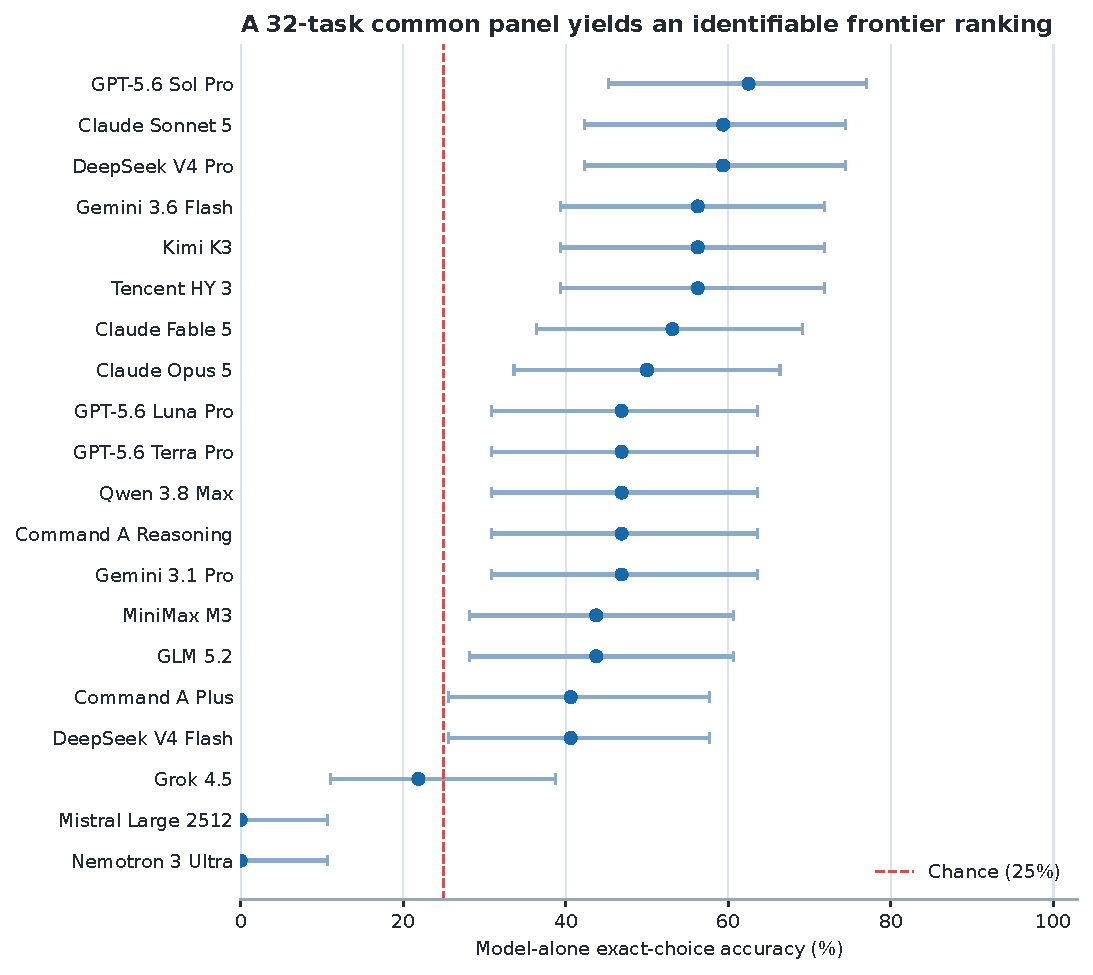
\includegraphics[width=0.88\linewidth]{figures/epicure-native/frontier-score-forest.pdf}
  \caption{Model-alone accuracy against \epicure{} answer keys. Points are exact accuracy over the
  common 32-task panel; bars are 95\% Wilson intervals. The dashed line is four-choice chance.}
  \label{fig:forest}
\end{figure*}

\begin{table*}[t]
  \centering
  \scriptsize
  \begin{tabular}{@{}r l r r r r r@{}}
\toprule
Rank & Model & FB Score & +Epicure & Gain & Model \% done & Epicure \% done \\
\midrule
1 & GPT-5.6 Sol Pro & 62.5 & 100.0 & +37.5 & 96.9 & 100.0 \\
2 & Claude Sonnet 5 & 59.4 & 100.0 & +40.6 & 100.0 & 100.0 \\
3 & DeepSeek V4 Pro & 59.4 & 93.8 & +34.4 & 100.0 & 93.8 \\
4 & Gemini 3.6 Flash & 56.2 & 100.0 & +43.8 & 100.0 & 100.0 \\
5 & Kimi K3 & 56.2 & 100.0 & +43.8 & 100.0 & 100.0 \\
6 & Tencent HY 3 & 56.2 & 100.0 & +43.8 & 100.0 & 100.0 \\
7 & Claude Fable 5 & 53.1 & 100.0 & +46.9 & 93.8 & 100.0 \\
8 & Claude Opus 5 & 50.0 & 100.0 & +50.0 & 100.0 & 100.0 \\
9 & GPT-5.6 Luna Pro & 46.9 & 100.0 & +53.1 & 100.0 & 100.0 \\
10 & GPT-5.6 Terra Pro & 46.9 & 100.0 & +53.1 & 100.0 & 100.0 \\
11 & Qwen 3.8 Max & 46.9 & 100.0 & +53.1 & 87.5 & 100.0 \\
12 & Command A Reasoning & 46.9 & 96.9 & +50.0 & 93.8 & 100.0 \\
13 & Gemini 3.1 Pro & 46.9 & 96.9 & +50.0 & 93.8 & 96.9 \\
14 & MiniMax M3 & 43.8 & 100.0 & +56.2 & 96.9 & 100.0 \\
15 & GLM 5.2 & 43.8 & 96.9 & +53.1 & 100.0 & 96.9 \\
16 & Command A Plus & 40.6 & 100.0 & +59.4 & 100.0 & 100.0 \\
17 & DeepSeek V4 Flash & 40.6 & 100.0 & +59.4 & 75.0 & 100.0 \\
18 & Grok 4.5 & 21.9 & 100.0 & +78.1 & 31.2 & 100.0 \\
DNF & Mistral Large 2512 & 0.0 & 93.8 & +93.8 & 0.0 & 100.0 \\
DNF & Nemotron 3 Ultra & 0.0 & 0.0 & +0.0 & 0.0 & 0.0 \\
\bottomrule
\end{tabular}

  \caption{The public 20-model leaderboard. ``Base'' is model-alone exact-choice accuracy;
  ``+Epicure'' is the matched tool-enabled accuracy; $\Delta$ is the percentage-point change;
  ``Base OK'' and ``Tool OK'' are parseable normal-completion rates in the two arms. Rank is
  determined by the model-alone Epicure Benchmark Score, with the published tie-breaks.}
  \label{tab:leaderboard}
\end{table*}

This is an automated model ranking, not a human preference table. The answer key exists before the
model call, every model receives the same questions, and all missing outputs remain incorrect. The
score can therefore be rerun as the roster changes without recruiting judges or prompting an LLM
evaluator.

The reliability columns separate culinary mistakes from execution failures. At the reliability
floor, \FBWorstBaseReliabilityModels{} emit a valid final marker on
\FBWorstBaseReliability\% of their arms. This is part of endpoint performance rather than
discarded noise: a response that never commits to A--D cannot solve an exact-choice task.

\subsection{What Epicure changes}

Across all 640 model--task pairs, accuracy moves from \FBAggregateOff\% without the tool to
\FBAggregateOn\% with it, an aggregate change of \FBAggregateUplift{} points. The average conceals
substantial heterogeneity: \FBPositiveUpliftModels{} models improve, \FBNegativeUpliftModels{}
decline, and \FBZeroUpliftModels{} are unchanged. \FBBestUpliftModel{} has the largest increase
(\FBBestUplift{} points); \FBWorstUpliftModel{} has the smallest change
(\FBWorstUplift{} points).

\begin{figure*}[t]
  \centering
  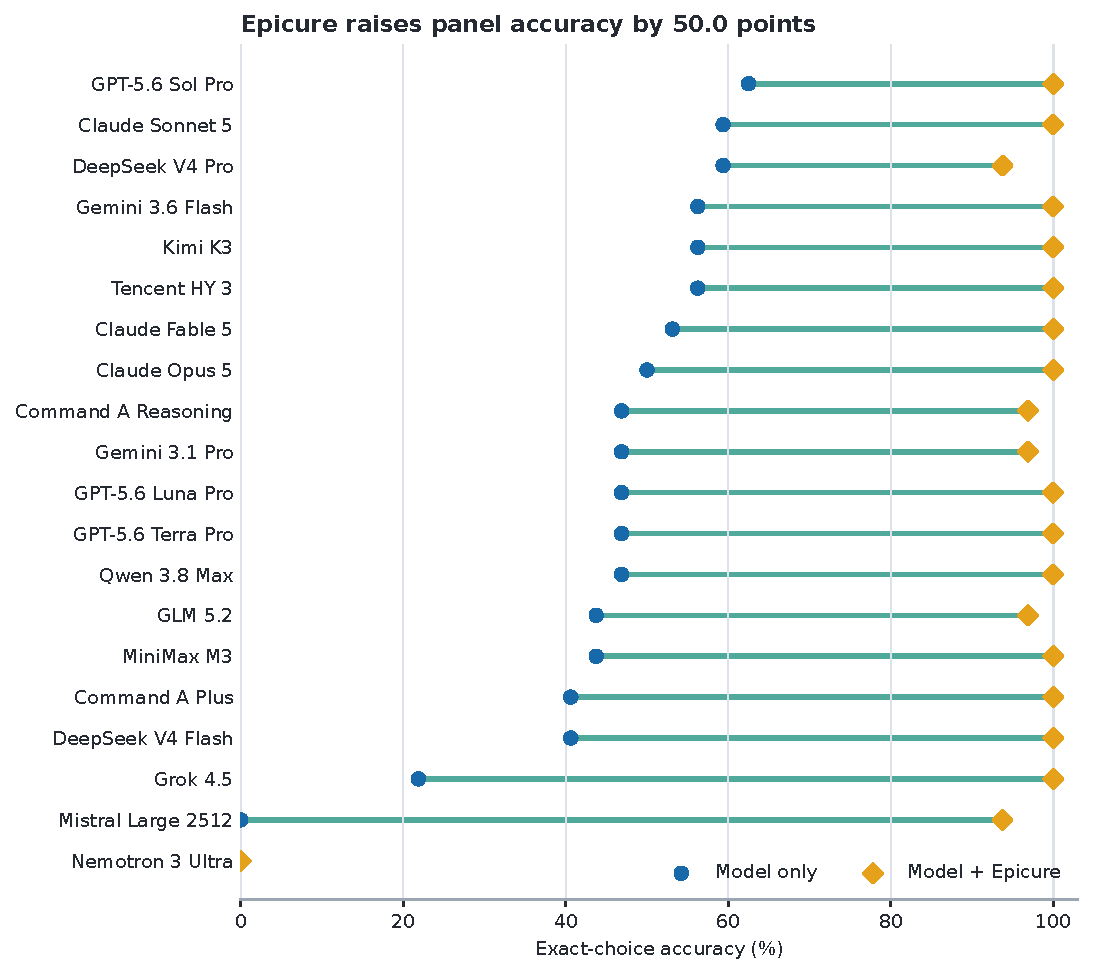
\includegraphics[width=0.88\linewidth]{figures/epicure-native/frontier-score-dumbbell.pdf}
  \caption{Matched model-alone and tool-enabled accuracy. The line segment for each model is an
  intervention contrast over the same 32 tasks, not a comparison between different samples.}
  \label{fig:dumbbell}
\end{figure*}

Tool access is not guaranteed to help. A model can select the wrong operation, copy the wrong field,
or abandon a correct prior belief after seeing an irrelevant result. Conversely, a model with weak
memorised culinary knowledge can recover the exact target when it chooses the reference operation.
The paired design exposes both behaviours.

\subsection{Families explain aggregate ties}

The four task families have different demands. Pairing questions require an exact four-decimal
value; substitution and cultural questions can sometimes be answered from broad food knowledge;
axis comparisons require a directional decision in \epicure{}'s latent space. \Cref{fig:heatmap}
shows that similar total scores can arise from different profiles.

\begin{figure*}[t]
  \centering
  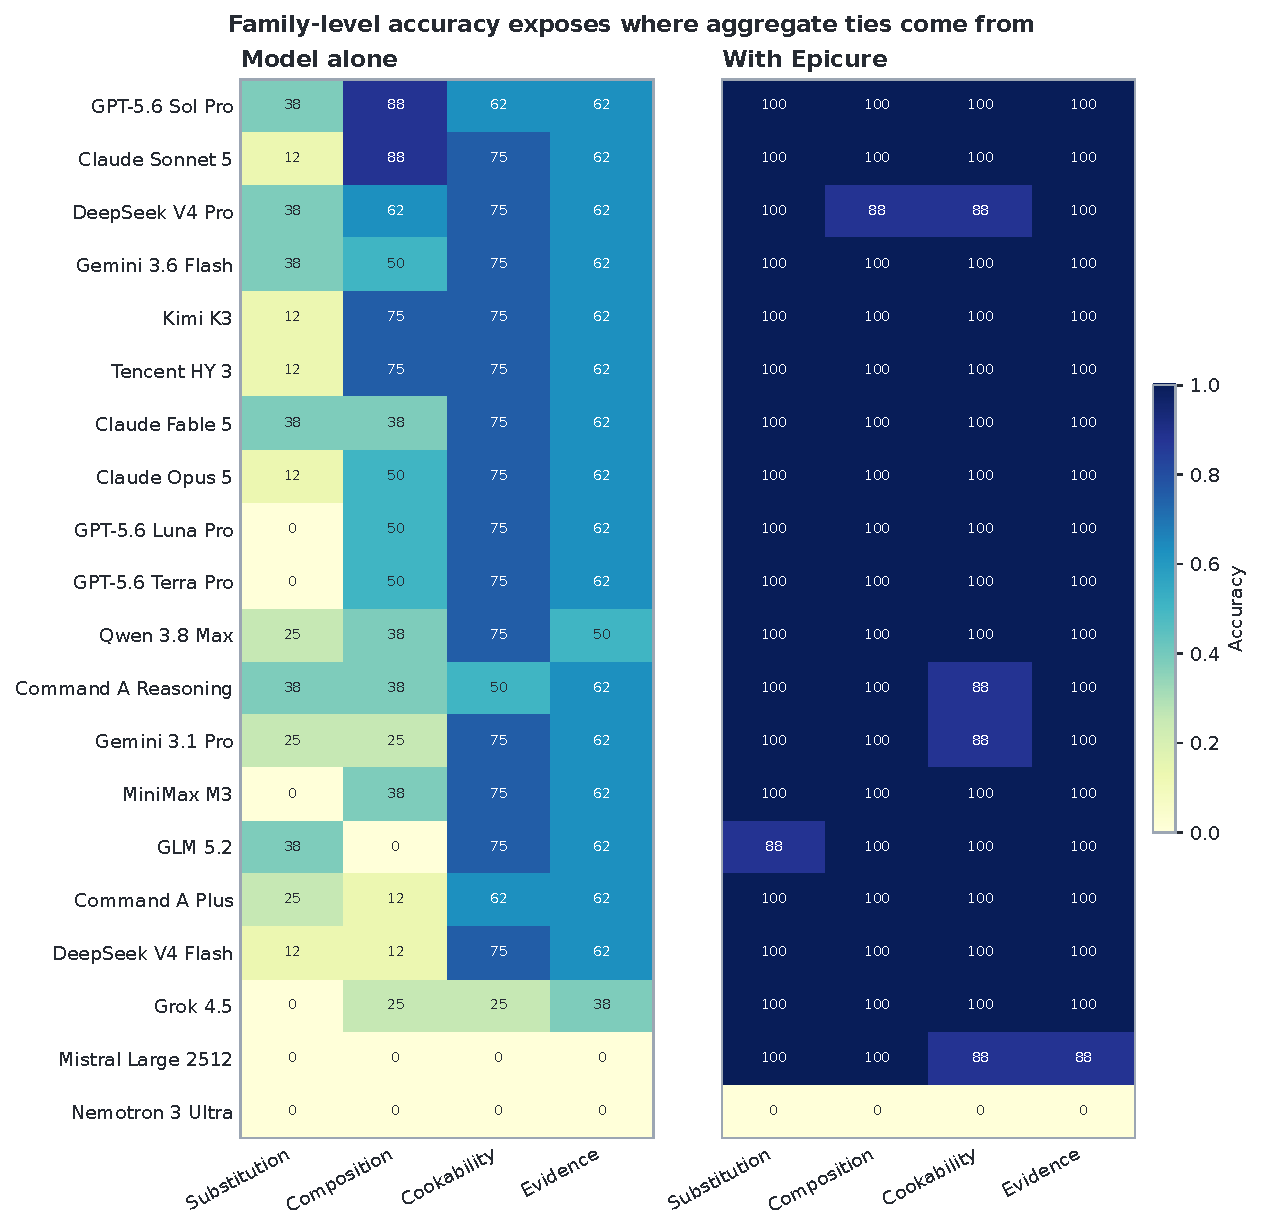
\includegraphics[width=0.95\linewidth]{figures/epicure-native/frontier-family-heatmap.pdf}
  \caption{Accuracy by model, condition, and task family. Values are percentages over eight tasks.
  The paired heatmaps show where tool access repairs a knowledge gap and where it introduces one.}
  \label{fig:heatmap}
\end{figure*}

\begin{table}[t]
  \centering
  \scriptsize
  \begin{tabular}{@{}l l r r r@{}}
\toprule
Family & Epicure operation & Tasks & Model only & Model + Epicure \\
\midrule
Substitution & \texttt{neighbors} & 8 & 18.1 & 94.4 \\
Composition & \texttt{pairing\_score} & 8 & 40.6 & 94.4 \\
Cookability & \texttt{compare\_on\_axis} & 8 & 62.5 & 92.5 \\
Evidence & \texttt{cultural\_profile} & 8 & 54.4 & 94.4 \\
\bottomrule
\end{tabular}

  \caption{Panel-average performance by family and the corresponding reference operation.}
  \label{tab:families}
\end{table}

\subsection{Every model--task pair is inspectable}

Aggregate bars can hide a benchmark bug or a single pathological task. \Cref{fig:matrix} therefore
publishes all 640 paired outcomes. Blue cells are stable knowledge: both conditions are correct.
Gold cells are direct tool wins. Red cells identify regressions after tool access. Grey cells show
questions neither condition solved.

\begin{figure*}[t]
  \centering
  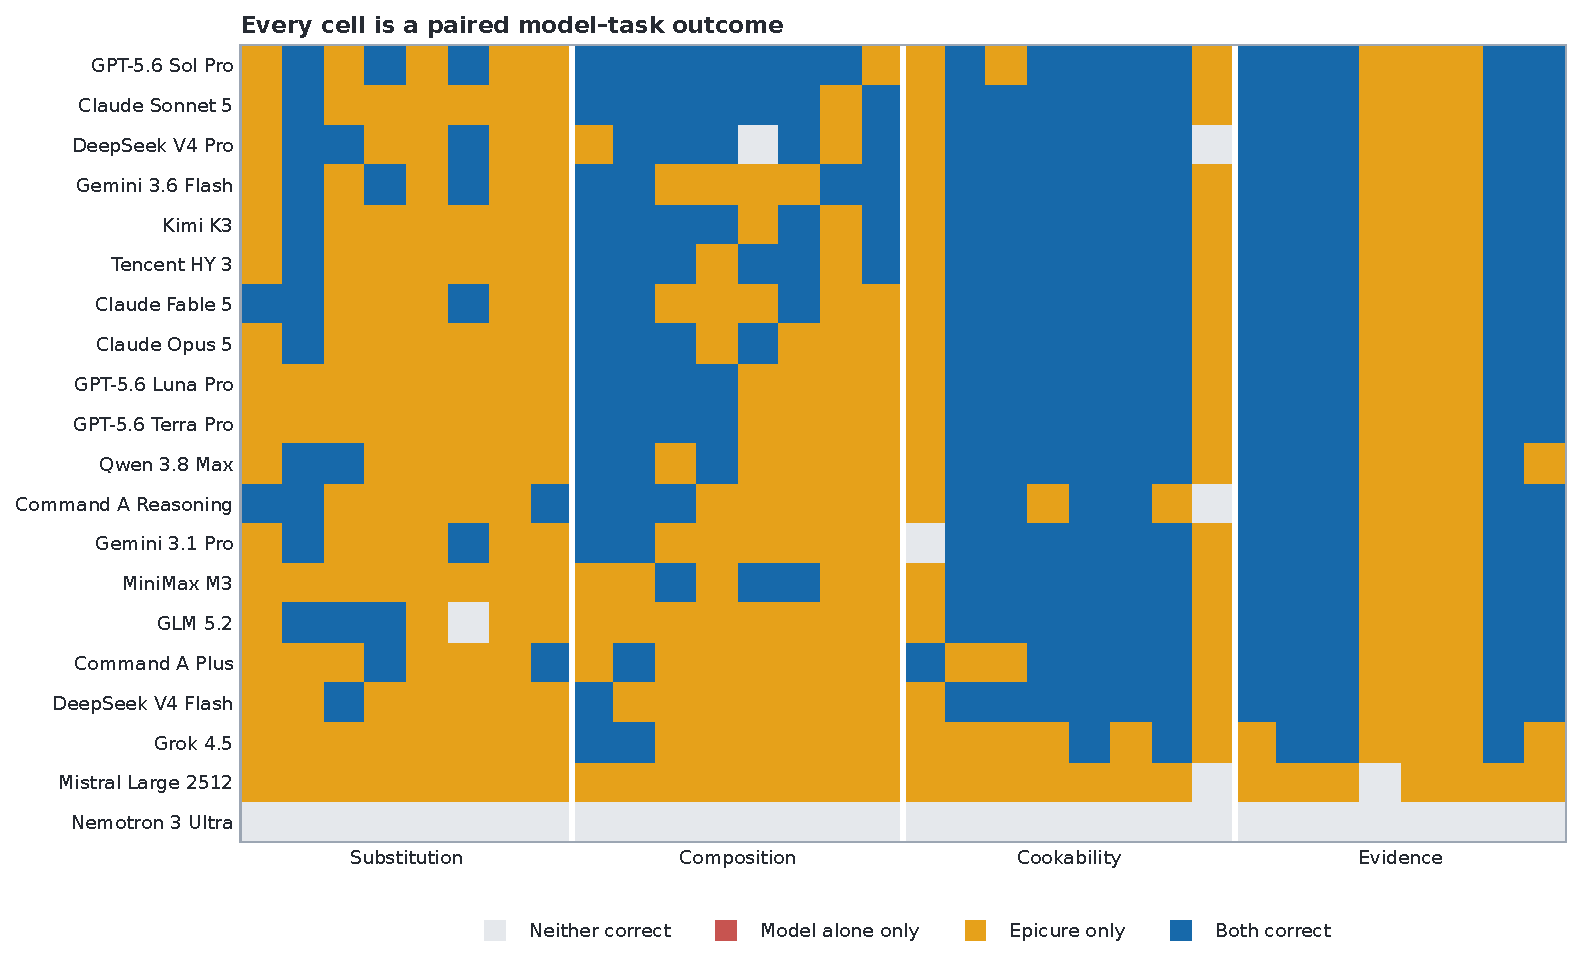
\includegraphics[width=\linewidth]{figures/epicure-native/frontier-paired-outcome-matrix.pdf}
  \caption{The complete $20\times32$ paired outcome matrix, ordered by public rank and grouped by
  task family. This is the most granular view of both benchmark difficulty and tool uplift.}
  \label{fig:matrix}
\end{figure*}

\subsection{Cohere, Kimi, Qwen, and route fidelity}

Both Cohere models are first-class members of the public panel, not appendix-only smokes. Command A
Plus is ranked \FBCoherePlusRank{} at \FBCoherePlusScore{} and changes by
\FBCoherePlusUplift{} points with \epicure{}; Command A Reasoning is ranked
\FBCohereReasoningRank{} at
\FBCohereReasoningScore{} and changes by \FBCohereReasoningUplift{} points. Kimi K3 is rank
\FBKimiRank{} through the direct Kimi endpoint. Qwen 3.8 Max is rank \FBQwenRank{} through an
explicit pay-as-you-go OpenRouter route, and GLM 5.2 is rank \FBGLMRank{}. No route silently
changes during generation.

The two direct Cohere routes each produced all 64 assigned arms. Their returned identifiers are
\texttt{\seqsplit{command-a-plus-05-2026}} and
\texttt{\seqsplit{command-a-reasoning-08-2025}}, respectively; the direct Kimi route likewise
produced all 64 arms under returned identifier \texttt{k3}. The offline verifier checks these
provider, identity, and arm-count contracts before accepting the release.

This matters because a model name is not a transport contract. The release stores the requested
model, returned model, provider, route, generation ID, latency, token counts, and response hash.
Direct and routed endpoints can therefore be analysed separately without pretending they are
interchangeable deployments.

\subsection{Accuracy, latency, and uplift are different axes}

\Cref{fig:latency} plots model-alone score against median arm latency. Marker colour encodes uplift.
A fast model can be inaccurate; a high-scoring model can receive little benefit from the tool; a
lower-ranked model can be the best candidate for tool augmentation. These are separate deployment
decisions, and the release preserves all three.

\begin{figure*}[t]
  \centering
  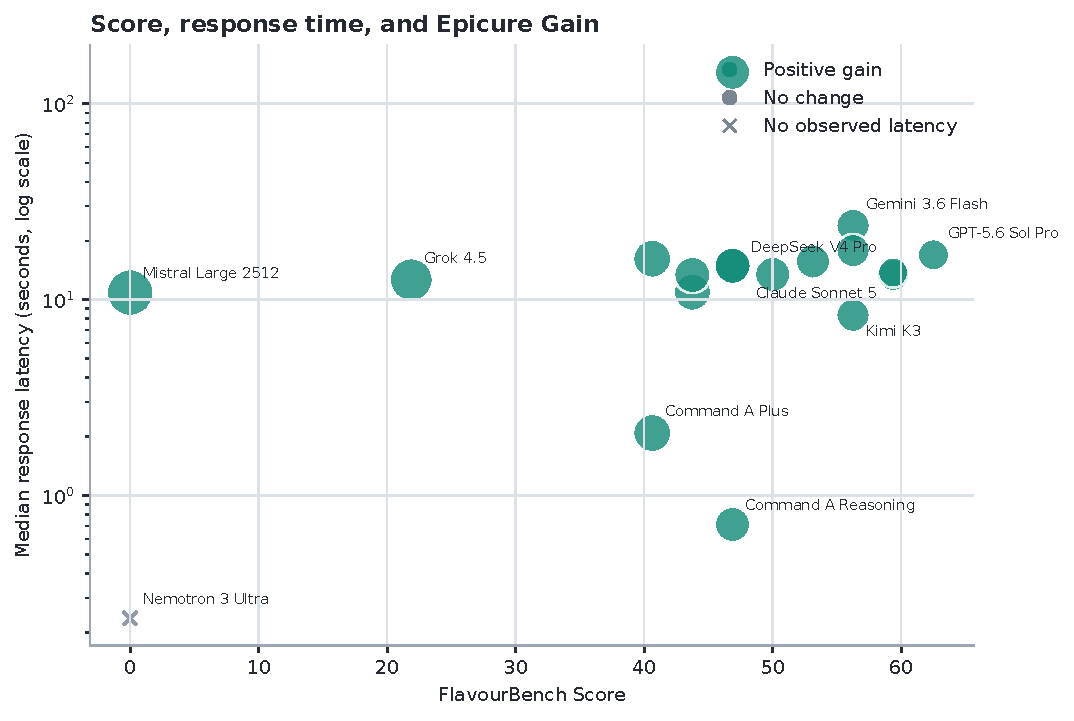
\includegraphics[width=0.82\linewidth]{figures/epicure-native/frontier-latency-uplift.pdf}
  \caption{Score, latency, and tool uplift. Latency uses a log scale. Point size increases with the
  magnitude of uplift; colour indicates its direction. An $\times$ marks a route with no observed
  latency.}
  \label{fig:latency}
\end{figure*}

\section{Real prompts, answers, and tool calls}
\label{sec:cases}

A benchmark paper should show what was actually asked. The four cases below are selected
mechanically, one per family. Where possible, the builder chooses a model--task pair that is wrong
without \epicure{} and correct with it. Each case includes the full prompt, both final answers, the
actual operation and arguments, and the exact answer key.

\paragraph{Case 1: Substitution with GPT-5.6 Sol Pro.}
\textbf{Prompt.} FlavourBench Epicure-native exact task. Use the read-only culinary evidence tools if they are available; otherwise answer from your own knowledge.

According to Epicure's `neighbors` result for `tomato` with top\_k=4, which ingredient is ranked first?

Choices:
A. oregano
B. bell\_pepper
C. olive\_oil
D. onion

In your final answer, explain briefly if useful and finish on its own line with exactly `FINAL\_CHOICE: X`, replacing X with A, B, C, or D.

\textbf{Model alone.} \texttt{FINAL\_CHOICE: D} \quad \textbf{With Epicure.} \texttt{FINAL\_CHOICE: B}

\textbf{Epicure call.} \texttt{neighbors}\allowbreak\texttt{(\{"ingredient": "tomato", "top\_k": 4\})}. The answer key is \texttt{FINAL\_CHOICE: B}.

\textbf{Epicure result.} {\ttfamily\footnotesize\sloppy \{"ingredient": "tomato", "neighbors": [\{"name": "bell\_pepper", "rank": 1, "sim": 0.4799\}, \{"name": "olive\_oil", "rank": 2, "sim": 0.4786\}, \{"name": "oregano", "rank": 3, "sim": 0.4646\}, \{"name": "onion", "rank": 4, "sim": 0.4567\}]\}}

\paragraph{Case 2: Composition with DeepSeek V4 Pro.}
\textbf{Prompt.} FlavourBench Epicure-native exact task. Use the read-only culinary evidence tools if they are available; otherwise answer from your own knowledge.

What exact four-decimal `pairing\_score` does Epicure return for `tomato` and `basil`?

Choices:
A. 0.2707
B. 0.2407
C. 0.3207
D. 0.1907

In your final answer, explain briefly if useful and finish on its own line with exactly `FINAL\_CHOICE: X`, replacing X with A, B, C, or D.

\textbf{Model alone.} \texttt{FINAL\_CHOICE: B} \quad \textbf{With Epicure.} \texttt{FINAL\_CHOICE: A}

\textbf{Epicure call.} \texttt{pairing\_score}\allowbreak\texttt{(\{"ingredient\_a": "tomato", "ingredient\_b": "basil"\})}. The answer key is \texttt{FINAL\_CHOICE: A}.

\textbf{Epicure result.} {\ttfamily\footnotesize\sloppy \{"all\_pairs\_range": \{"median": 0.092, "p10": 0.0197, "p25": 0.0521, "p75": 0.1392, "p90": 0.1899\}, "pairing\_score": 0.2707, "percentile\_label": "very high (>=p90)", "resolved\_a": "tomato", "resolved\_b": "basil"\}}

\paragraph{Case 3: Cookability with GPT-5.6 Sol Pro.}
\textbf{Prompt.} FlavourBench Epicure-native exact task. Use the read-only culinary evidence tools if they are available; otherwise answer from your own knowledge.

Which statement matches Epicure's `compare\_on\_axis` result for `coffee` versus `chocolate` on `cf\_bitter`?

Choices:
A. coffee has the higher projection
B. the projections are equal to four decimals
C. Epicure cannot resolve one or both ingredients
D. chocolate has the higher projection

In your final answer, explain briefly if useful and finish on its own line with exactly `FINAL\_CHOICE: X`, replacing X with A, B, C, or D.

\textbf{Model alone.} \texttt{FINAL\_CHOICE: A} \quad \textbf{With Epicure.} \texttt{FINAL\_CHOICE: D}

\textbf{Epicure call.} \texttt{compare\_on\_axis}\allowbreak\texttt{(\{"axis": "cf\_bitter", "ingredient\_a": "coffee", "ingredient\_b": "chocolate"\})}. The answer key is \texttt{FINAL\_CHOICE: D}.

\textbf{Epicure result.} {\ttfamily\footnotesize\sloppy \{"axis": "cf\_bitter", "axis\_range": \{"p10": -0.0877, "p90": 0.1429\}, "delta": 0.0835, "label\_a": "moderate", "label\_b": "high", "projection\_a": 0.0076, "projection\_b": 0.0911, "resolved\_a": "coffee", "resolved\_b": "chocolate"\}}

\paragraph{Case 4: Evidence with Grok 4.5.}
\textbf{Prompt.} FlavourBench Epicure-native exact task. Use the read-only culinary evidence tools if they are available; otherwise answer from your own knowledge.

Which cuisine direction has the highest cosine score in Epicure's `cultural\_profile` result for `miso`?

Choices:
A. Japanese
B. East\_Asian
C. Southeast\_Asian
D. South\_Asian

In your final answer, explain briefly if useful and finish on its own line with exactly `FINAL\_CHOICE: X`, replacing X with A, B, C, or D.

\textbf{Model alone.} \texttt{\{"name": "cultural\_profile", "arguments": \{"ingredient": "miso"\}\}} \quad \textbf{With Epicure.} \texttt{FINAL\_CHOICE: A}

\textbf{Epicure call.} \texttt{cultural\_profile}\allowbreak\texttt{(\{"ingredient": "miso"\})}. The answer key is \texttt{FINAL\_CHOICE: A}.

\textbf{Epicure result.} {\ttfamily\footnotesize\sloppy \{"cuisines": \{"East\_Asian": \{"range": \{"p10": -0.1649, "p90": 0.3039\}, "score": 0.1625\}, "Eastern\_European": \{"range": \{"p10": -0.1466, "p90": 0.1034\}, "score": -0.1494\}, "Japanese": \{"range": \{"p10": -0.1359, "p90": 0.1896\}, "score": 0.3227\}, "Latin\_American": \{"range": \{"p10": -0.1672, "p90": 0.1281\}, "score": -0.1538\}, "Mediterranean": \{"range": \{"p10": -0.2323, "p90": 0.206\}, "score": -0.1198\}, "South\_Asian": \{"range": \{"p10": -0.0808, "p90": 0.071\}, "score": -0.0585\}, "Southeast\_Asian": \{"range": \{"p10": -0.1625, "p90": 0.193\}, "score": 0.0426\}, "Western\_Atlantic": \{"range": \{"p10": -0.2304, "p90": 0.183\}, "score": -0.1546\}\}, "note": "Cosine similarity to each cuisine direction. Use p10/p90 to judge whether a score is typical or extreme.", "resolved": "miso"\}}


These examples make the construct visible. The model-alone arm tests knowledge or inference about
the hidden graph. The tool-enabled arm tests whether the model can identify the relevant operation,
form valid arguments, read the returned structure, and preserve the answer contract. A correct
choice with the wrong operation still earns answer credit, but the release separately reports
whether the reference operation was matched. Across the run there are \FBToolCalls{} projected
\epicure{} calls and \FBReferenceMatches{} model--task pairs matching the reference operation.

\section{From benchmark score to training reward}
\label{sec:training}

The same environment can supervise more than a leaderboard. For each generated trajectory $\tau$,
define four deterministic components:
\begin{align}
 r_{\mathrm{answer}}(\tau) &= \mathbb{1}[\hat y(\tau)=y_t],\\
 r_{\mathrm{format}}(\tau) &= \mathbb{1}[\text{normal parseable final}],\\
 r_{\mathrm{call}}(\tau) &= \mathbb{1}[\text{successful Epicure call}],\\
 r_{\mathrm{align}}(\tau) &= \mathbb{1}[\text{reference call matches}].
\end{align}
The public leaderboard uses $r_{\mathrm{answer}}$ in the model-alone condition. A tool-agent reward
can use
\begin{equation}
 r(\tau)=r_{\mathrm{answer}}r_{\mathrm{format}}
 +\lambda r_{\mathrm{answer}}r_{\mathrm{call}}
 +\mu r_{\mathrm{align}},
 \label{eq:reward}
\end{equation}
with $\lambda$ and $\mu$ chosen for the training objective. The answer term prevents reward hacking
through irrelevant tool calls; the alignment term distinguishes reaching the right answer by the
intended evidence path from accidental success.

Three training regimes follow naturally. \textbf{Rejection sampling} generates multiple responses
and retains exact successes. \textbf{Preference optimisation} pairs a successful trajectory with a
failed response to the same task and model checkpoint. \textbf{Reinforcement learning} queries the
runtime online and uses \Cref{eq:reward} as a verifiable reward. New ingredient seeds create fresh
tasks, which reduces direct memorisation of the published 32-item panel.

This paper releases the executable reward interface and the paired evidence that motivates it;
training a new checkpoint is the next experiment. That experiment should use disjoint generated
seeds and keep the public leaderboard as a final evaluation split.

\section{Reproducibility and release}
\label{sec:reproduction}

The public release is one JSON document with hash \FBReleaseSHA{}. It contains the 20 route records,
32 full prompts, answer keys and reference \epicure{} results, 1,280 observation rows, final answer
markers, latency and cost fields, and bounded tool-trace projections. \FBObservedArms{} provider
responses were observed; \FBMissingArms{} missing arms remain explicit zero-scored rows.

The leaderboard can be reconstructed without a network connection, provider key, GPU, or running
\epicure{} service:

\begin{verbatim}
python3 -I reproduce_epicure_native.py \
  --release generated/epicure-native/\
  epicure-native-release.json
\end{verbatim}

The verifier rejects duplicate JSON keys, non-finite numbers, a changed content address, an
incomplete $20\times32\times2$ grid, or any leaderboard value that differs from recomputation. The
paper tables and figures are generated from the same release, so a changed score cannot leave a
stale chart behind.

Reproducing the original hosted calls is a different operation from replaying the result. The
release records exact routes and request policies, but provider deployments can change. A fresh
frontier run should generate a new manifest and release rather than overwrite this snapshot.

\section{Discussion}
\label{sec:discussion}

\paragraph{What the rank means.}
The Epicure Benchmark Score measures how often a model can recover answers defined by a published
culinary runtime. It is not a universal measure of cooking skill. Its value is that the target is
clear, model-independent, and executable. The four families make the ranking broader than one API
call while keeping every item auditable.

\paragraph{Do we need humans?}
Not for this leaderboard. Humans are useful when the target is preference, creativity, safety, or
the quality of an open-ended recipe. They are unnecessary when the question is whether a model's
choice matches a deterministic runtime result. \system{} uses that distinction to automate the
core ranking while leaving subjective culinary evaluation as a separate track.

\paragraph{Why pair tool access?}
A standalone benchmark says which model best predicts \epicure{}. The paired intervention says
whether \epicure{} itself helps each model. That second result is operationally important: a strong
base model may ignore tools, while a weaker model may become competitive when grounded. The
dumbbell and pair matrix expose this directly.

\paragraph{Scaling the benchmark.}
The current task compiler can generate more items by expanding seed lists while preserving the
same four operations. A larger release should reserve unseen ingredients and pairs, deduplicate
near-equivalent questions, and measure stability across runtime versions. The public 32-task panel
is best viewed as a frontier snapshot and a reproducible template for larger hidden sets.

\section{Related work}

HELM argues for explicit scenarios and metrics, while recent benchmark audits emphasise validity,
contamination, and transparent reporting \cite{liang2022helm,reuel2024betterbench}. Chatbot Arena
and WildBench evaluate broad answer quality through preferences or checklists
\cite{chiang2024chatbotarena,lin2024wildbench}. \system{} instead targets an executable domain model
and needs no judge for its primary score.

ToolLLM, BFCL, and $\tau$-bench make tool invocation or environment state observable
\cite{qin2023toolllm,patil2025bfcl,yao2024taubench}. \system{} adds a matched no-tool condition, so
tool access becomes an intervention rather than a requirement shared by every arm. LiveBench,
LiveCodeBench, GPQA, MMLU-Pro, and SWE-bench illustrate complementary strategies for reducing
contamination or grounding answers in difficult tasks and executable outcomes
\cite{white2024livebench,jain2024livecodebench,rein2023gpqa,wang2024mmlupro,jimenez2023swebench}.

\begin{table*}[t]
  \centering
  \small
  \begin{tabularx}{\linewidth}{@{}l l X c c@{}}
    \toprule
    Benchmark & Scope & Per-answer target & Deterministic score & Matched tool contrast \\
    \midrule
    Chatbot Arena & general chat & pairwise human preference & No & No \\
    WildBench & general chat & checklist-guided model judgment & No & No \\
    BFCL & function calling & structured call correctness & Yes & No \\
    $\tau$-bench & interactive agents & environment goal state & Yes & No \\
    \system{} & culinary agents & versioned \epicure{} operation & Yes & Yes \\
    \bottomrule
  \end{tabularx}
  \caption{\system{} complements broad preference and tool-use benchmarks. Its distinctive unit is
  the same model--task pair measured without and with the domain oracle that generated the answer.}
  \label{tab:benchmark-comparison}
\end{table*}

Culinary datasets such as FlavorDB and Recipe1M organise ingredient and recipe evidence
\cite{garg2018flavordb,salvador2017recipe1m}. CookingSense and planning-oriented culinary work test
commonsense and procedural reasoning \cite{choi2024cookingsense,wu2025recipe2plan}. \epicure{}
occupies a different layer: it exposes a callable structured representation whose outputs can be
compiled into exact evaluation targets.

\section{Limitations}

The published panel has 32 tasks and therefore resolves large score differences better than close
ones. The ingredient seeds are English identifiers and cover only four \epicure{} operations.
Hosted model routes are a dated snapshot, and identical public prompts can eventually be memorised.
Finally, agreement with \epicure{} inherits the runtime's representation choices; it should not be
read as a food-safety or cultural-authenticity certification.

These limits have direct remedies: generate held-out seeds, add runtime operations, report multiple
versioned panels, and keep subjective recipe-quality evaluation separate. None requires replacing
the exact automated score with an opaque judge.

\section{Conclusion}

\system{} supplies a public automated leaderboard for culinary agents. \epicure{} creates the
questions, fixes the answers, and serves as the paired tool intervention. On the 20-model common
panel, \FBTopModel{} ranks first at \FBTopScore{} and \FBBottomModel{} ranks twentieth at
\FBBottomScore{}. Tool access changes panel accuracy by \FBAggregateUplift{} points, with strongly
model-dependent effects. Every number is recoverable from the released 1,280-arm grid.

The broader result is architectural: a domain model can be more than a retrieval plugin. When its
outputs are deterministic and versioned, it becomes an oracle for evaluation and a reward source
for learning. \system{} demonstrates that loop end to end.

\appendix

\section{Exact execution routes}
\label{app:routes}

\begin{table*}[h]
  \centering
  \scriptsize
  \begin{tabular}{@{}r l l@{}}
\toprule
Slot & Model & Execution route \\
\midrule
1 & GPT-5.6 Sol Pro & openrouter: openai/flex \\
6 & Claude Sonnet 5 & openrouter: amazon-bedrock/claude-on-aws \\
13 & DeepSeek V4 Pro & openrouter: baidu/fp8 \\
8 & Gemini 3.6 Flash & openrouter: google-vertex/global/flex \\
10 & Kimi K3 & kimi\_direct: kimi-code-direct \\
18 & Tencent HY 3 & openrouter: baidu/fp8 \\
4 & Claude Fable 5 & openrouter: amazon-bedrock \\
5 & Claude Opus 5 & openrouter: amazon-bedrock/claude-on-aws \\
3 & GPT-5.6 Luna Pro & openrouter: openai/flex \\
2 & GPT-5.6 Terra Pro & openrouter: openai/flex \\
11 & Qwen 3.8 Max & openrouter: alibaba \\
20 & Command A Reasoning & cohere\_direct: cohere-direct \\
7 & Gemini 3.1 Pro & openrouter: google-vertex/global/flex \\
15 & MiniMax M3 & openrouter: together \\
12 & GLM 5.2 & openrouter: coreweave/fp4 \\
19 & Command A Plus & cohere\_direct: cohere-direct \\
14 & DeepSeek V4 Flash & openrouter: cloudflare/fp8 \\
9 & Grok 4.5 & openrouter: xai/zdr \\
17 & Mistral Large 2512 & openrouter: mistral \\
16 & Nemotron 3 Ultra & openrouter: deepinfra/fp4 \\
\bottomrule
\end{tabular}

  \caption{All 20 model routes in the released leaderboard. Routes are selected before generation;
  automatic fallback is disabled.}
  \label{tab:routes}
\end{table*}

\section{Protocol details}

All arms request temperature 0, top-$p$ 1, and seed 20260810 where the provider supports it. The
final response budget is 2,048 tokens. The tool-enabled arm has one tool round, one call total, a
4,096-byte result bound, and a 4,096-byte cumulative result bound. At most two provider attempts
are allowed, and an ambiguously delivered request is never replayed. The final marker is parsed
from plain text for transport portability; direct providers may use native structured generation
internally and normalize to the same marker.

\section{Data fields}

Each observation binds model ID, task ID, condition, source status, source and response hashes,
returned model and provider, finish reason, latency, cost, final answer, observed and expected
choice, normal-parse flag, correctness, and a projected tool trace. Each tool event contains its
name, structured arguments, error flag, latency, and result hash. The release does not require raw
provider credentials or hidden service state.

% Flush benchmark figures and appendix tables before the references so the
% empirical story remains contiguous in the compiled paper.
\clearpage
\bibliographystyle{plain}
\bibliography{references}

\end{document}
